\section{Implementation}
\label{sec:implementation}

\subsection{System Design}

Backscattered light from an object hit by a laser, like a speckle pattern, is typically very low in intensity. How low depends on the situation.

The light intensity $I_b$ at a distance $d$ is proportional to the laser power and decays quadratically with distance and can be calculated using a simplified model:

\begin{equation}
I_b = \frac{P \cdot \rho}{2\pi d^2},
\end{equation}
where:
\begin{itemize}
\item $P$ is the power of the incident laser beam, measured in watts (W),
\item $\rho$ is the reflectivity of the surface (unitless),
\item $d$ is the distance from the scattering surface to the photodiode, measured in meters (m).
\end{itemize}


\subsection{How much current?}
A photodiode converts the backscattered light intensity into current:
\begin{equation}
I_{\text{photo}} = I_b \cdot A_{\text{PD}} \cdot R,
\end{equation}
where:
\begin{itemize}
\item $I_b$ is the incident intensity at distance $d$ \text{(W/mm\textsuperscript{2})},
\item $A_{\text{PD}}$ is the area of the photodiode \text{(mm\textsuperscript{2})},
\item $R$ is the photodiode responsivity \text{(A/W)}.
\end{itemize}
Using typical values like $R = 0.5\text{A/W}$, $A_{\text{PD}} = 2\text{ mm}^2$, $P = 1\text{ mW}$ and $d = 0.3\text{ m}$ we are left with tiny photocurrents in the $500\text{ pA}$ range!

Therefore, a low noise and high gain first stage amplifier becomes necessary to achieve a workable output signal. 

To be certain, we conduct a small set of experiments (setup is shown in Figure \ref{fig:cam1}) to measure the current produced by a photodiode exposed to incident laser speckle pattern.

A typical store-bought class 1 red laser pointer has an output power under 0.5mW. 
Using this laser pointer and the Thorlabs PDA36A2 photodector (with a photodiode area: $A_{\text{PD}} = 13\text{ mm}^2$ and same $d$ as above), we observe ~13 ~nA of current.
This means that we need to at least be able to measure currents on this order of magnitude for class 1 lasers at ~30 ~cm distance.


\subsection{How big a photodiode?}
Can we test if a photodiode of a given size can be sensitive to a speckle pattern in motion? Recall that the sensor must be smaller than the speckle size in order to resolve speckle motion. Using the formula for mean speckle size, assuming a red laser at 650 ~nm and 30 ~cm distance, we find the resulting mean size to be around 100 ~um. This is too small for common photodiodes, but we make the assumption - based on observations of real speckle patterns - that the variance in size is large.

To validate this assumption, we masked the detector with a 0.9mm x 0.9mm pinhole on copper tape to cover the aperture of the detector (inspired by \cite{veber2011laserMASK}). 
We set the surface in motion and observed the output on a multimeter as well as on camera. As the speckle oscillated on camera, so did the multimeter output.

On Digikey, found the most sensitive, small, low cost photodiode: the VEMD2704 by Vishay with an area of $1.5\text{ mm}^2$.


\begin{figure}[t]
  \centering
  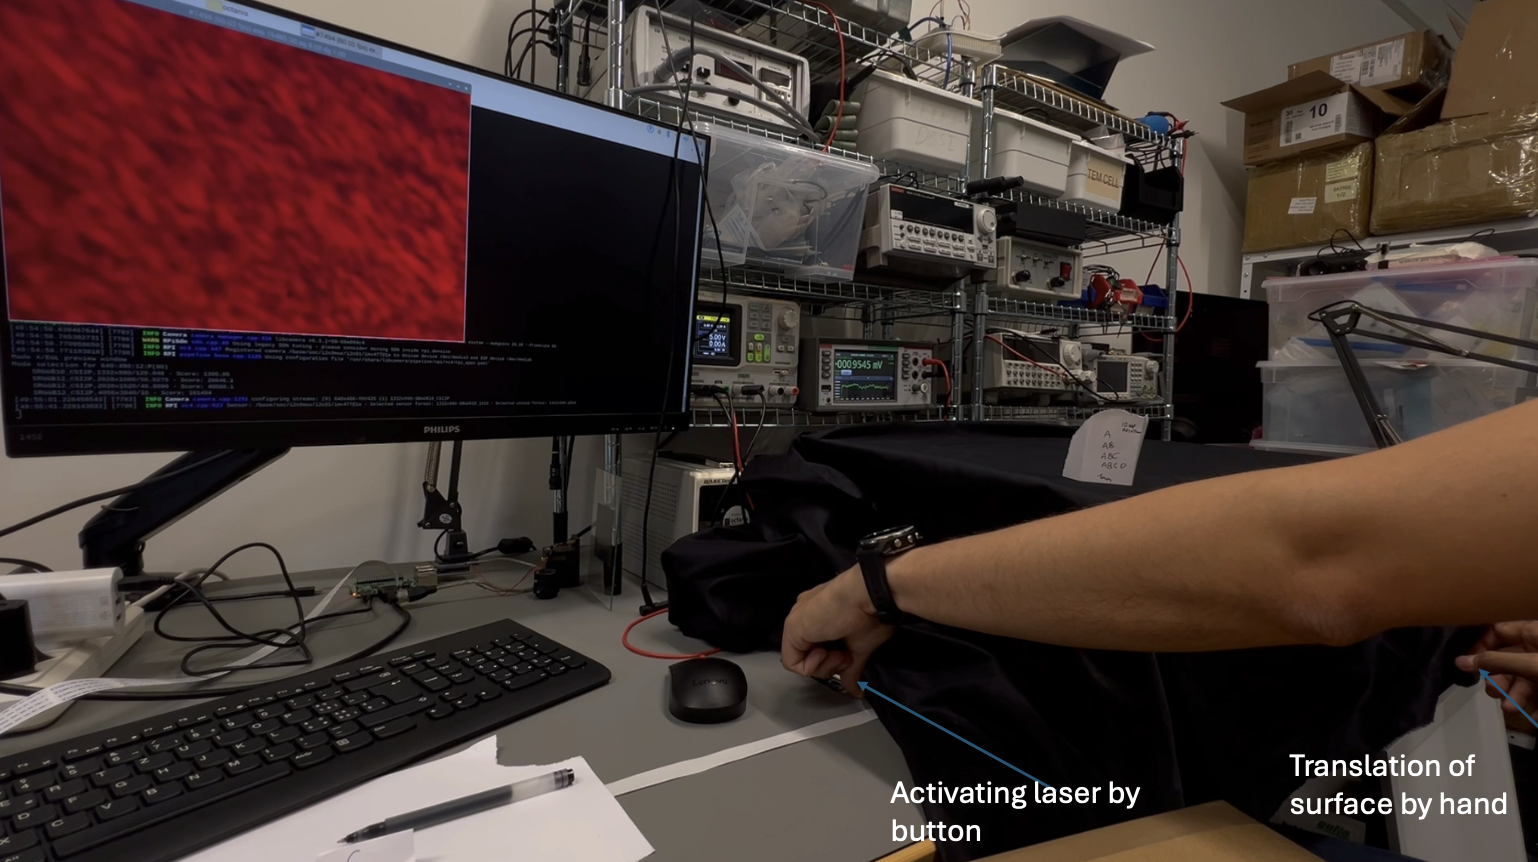
\includegraphics[width=\widthnarrow]{figures/impl/camera_setup2.png}
  \caption{Speckle pattern visualised by RPI Cam HQ (from Setup in Figure \ref{fig:cam1})}
  \label{fig:cam2}
\end{figure}

We make the following observations:
\begin{itemize}
  
  \item A CMOS sensor pixel is a photodiode and has as determined size.
  \item We can emulate the output of a larger photodiode by integrating over all pixels over the same area as the larger photodiode.
  \item The sensor area of the RPI camera is large enough to accomodate 9 VEMD2704 photodiodes (see Figure \ref{fig:emulated2}).
\end{itemize}

Using this knowledge, we record a video of a speckle pattern in motion and cut out the pixels corresponding to a grid of areas the same sizes as the VEMD2704. 
We establish that an algorithm similar to the one used by Streli et al \cite{structured-light-speckle} can be used to combine the outputs of the photodiodes in order to create a 1d motion signal.
Figure \ref{fig:emulated2} shows the resulting 1d signal of motion. The section on Signal Processing discusses this in detail.

\subsection{Hardware Implementation}

The system block system block diagram is given in \ref{fig:block} using the order of magnitude values devised in the initial experiments.
\begin{figure}[t]
  \centering
  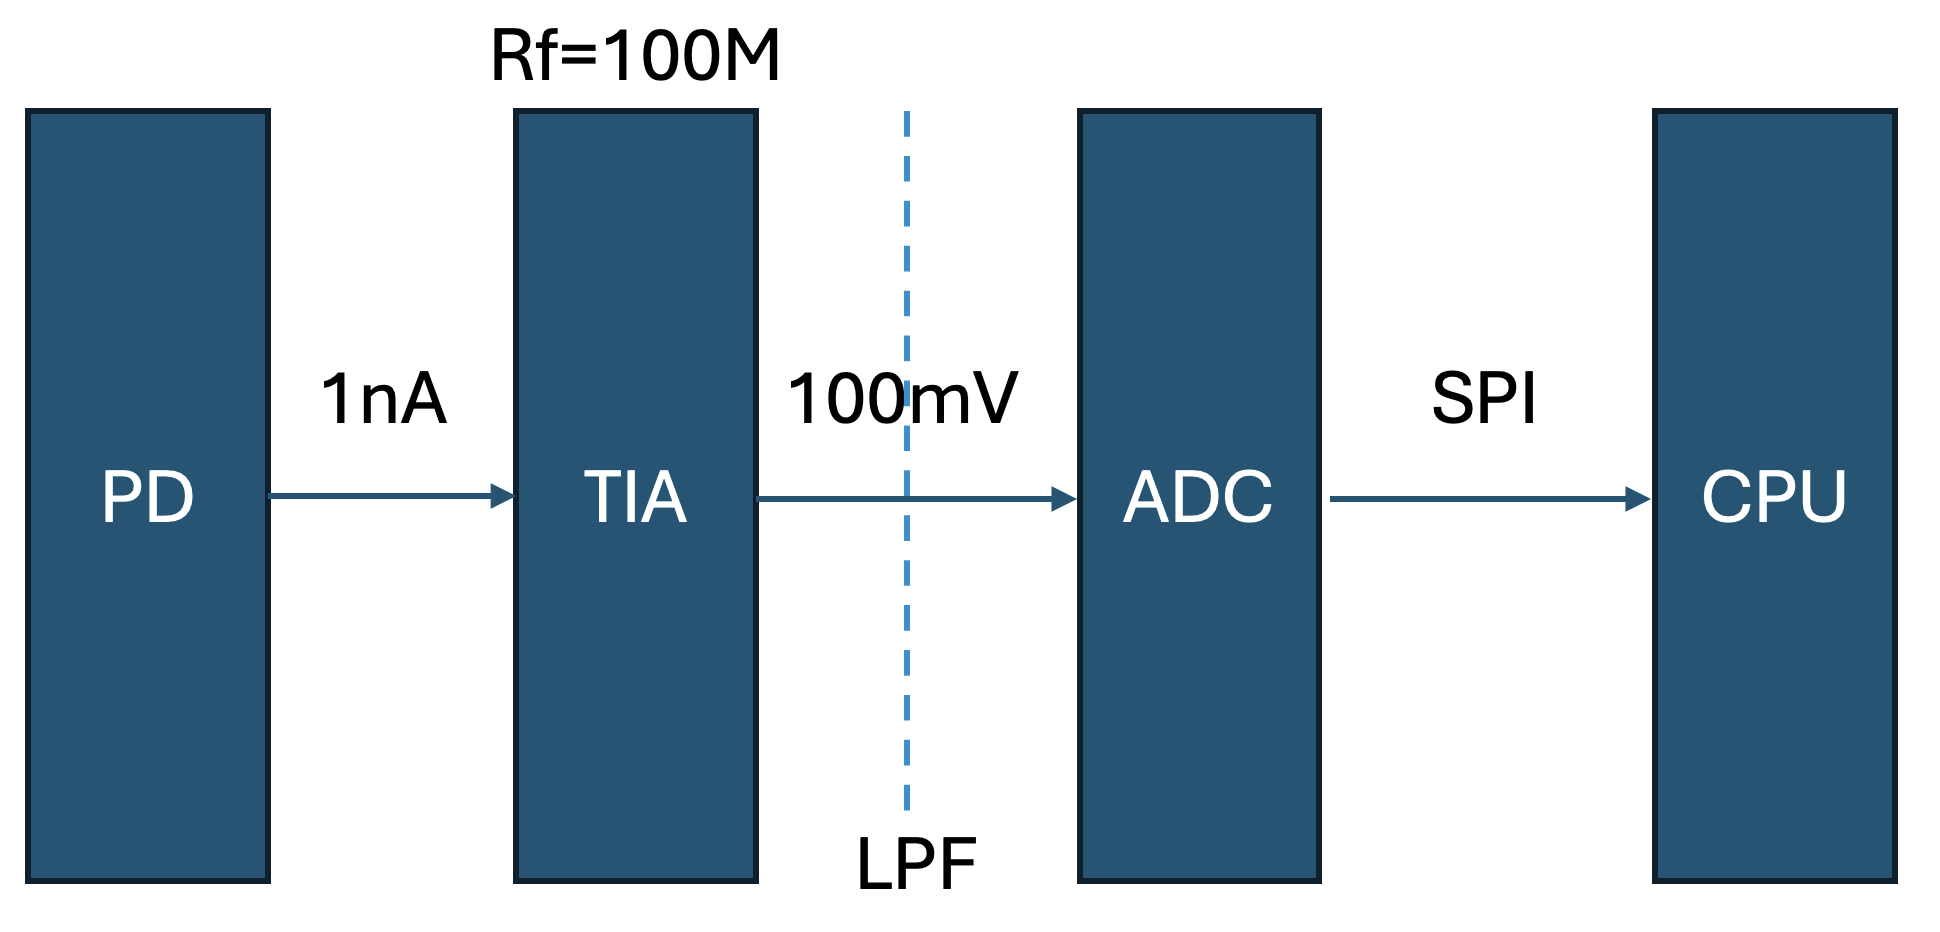
\includegraphics[width=\widthnarrow]{figures/impl/block_diagram.png}
  \caption{Block diagram}
  \label{fig:block}
\end{figure}

Photodiodes are commonly amplified using a transimpedance amplifier (TIA), although alternative options exist, such as current integrators like the DDC118. 
This application focuses on capturing high-frequency signals of up to 1 kHz, necessitating specific requirements for the operational amplifiers used.

%add formula from Op Amp Bandwidth for Transimpedance Amplifiers.pdf

The essential requirements for the op-amps include:
\begin{itemize}
  \item A minimum of two op-amps in a single package.
  \item A target price of approximately \$5 per chip.
  \item JFET input with low input bias current.
  \item Capability to operate on a single power supply.
\end{itemize}

The OPA2380 fulfilled these requirements and a PCB was designed and built according to the datasheet recommendations. Coupled with the VEMD2704 and a 100 MOhm feedback resistor, we can achieve 
Particular attention to leakage currents was taken, like the implementation of a guard ring. The guard ring is a low impedance path for any stray AC that might want to make its way into the feedback path of the amp. The PCB is shown in Figure \ref{fig:teaser} and contains a modular photodiode array with bandpass filter.

The bandpass filter is chosen to be at 850nm as that is where silicon photodiodes are most efficient. Lasers are 850nm are common and we are able to filter out a lot of environmental light.


\subsection{Signal Processing}

In this project, a Raspberry Pi 5 (RPI) was used with two types of Analog-to-Digital Converters (ADC).

The first ADC was unable to sample at high enough frequencies. Although it utilized a multiplexer (MUX), the channel switching was controlled via SPI, making it challenging to manage the switching delay. This limitation introduced a significant amount of noise, which was also noted in several GitHub issues reported by users.

A second ADC was then tested, featuring a higher sample rate and advertised synchronous sample readout capability. This ADC is designed as a Raspberry Pi HAT and uses the Pi's 5V supply as its analog reference. However, this reference is very noisy, with peak-to-peak noise in the millivolt range. To mitigate this issue, a bench power supply was used to power the ADC externally.

To convert the 9-channel photodiode array readings into a single vibrometry signal, we compute the inter-channel variance, explained later on. 
First, we remove common-mode fluctuations by subtracting the instantaneous mean across all channels:

\begin{equation}
s_i(t) = r_i(t) - \frac{1}{n}\sum_{k=1}^{n} r_k(t)
\end{equation}

where $r_i(t)$ is the raw intensity reading from channel $i$ and $n=9$ is the number of channels. We then compute the inter-channel variance:

\begin{equation}
V(t) = \frac{2}{n(n-1)} \sum_{i=1}^{n-1} \sum_{j=i+1}^{n} |s_i(t) - s_j(t)|
\end{equation}

This metric quantifies the average magnitude of pairwise intensity differences between spatial channels in the instantaneous speckle pattern. 
Changes in $V(t)$ over time indicate surface motion and vibration while being robust to common-mode noise.

Raw data from the ADC was recorded and observed in real-time or processed post-capture. 
Real-time observations were conducted while simultaneously monitoring the speckle camera and the infrared (IR) camera.

\begin{figure*}[t]
  \centering
  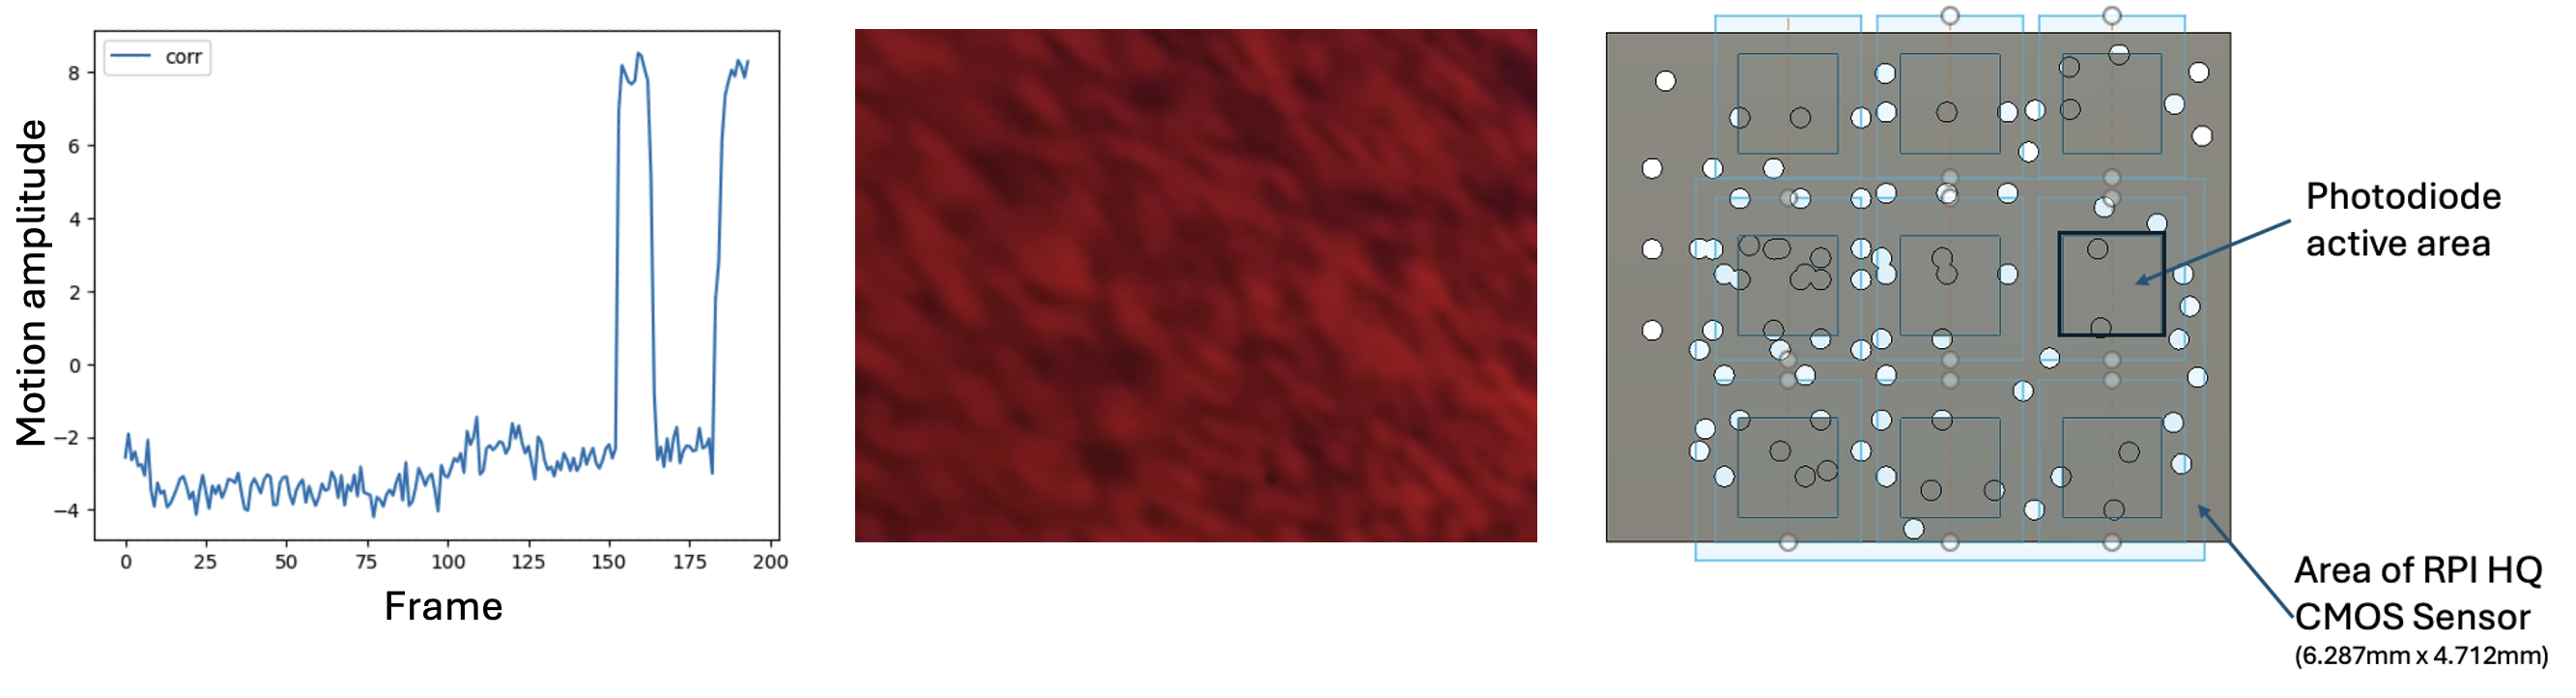
\includegraphics[width=\textwidth]{figures/impl/emulated2.png}
  \caption{Left to right: Peaks show translation of speckle pattern, signifying a change of the inter-channel variance. The speckle pattern on the camera sensor. The camera sensor with an overlayed photodiode grid.}
  \label{fig:emulated2}
\end{figure*}


\subsection{Lasers}

Several laser sources were built in different configurations as seen in Figure~\ref{fig:lasers}. 
The laser module used for the square array, circular array and single laser measurements is an 850~nm laser (VLM-850-03 by Quarton Inc.).
The Realsense D415 Depth Camera (by Intel) has a laser dot projector that can be turned on using the Realsense Viewer Software. 
To control the amount of laser dots that are output by the Realsense dot projector, an iris diaphragm (Edmund Optics 53906) is used.

Additionally, we reverse engineered the Realsense through visual inspection and found it to look very similar, if not identical, to the BELICE projector module by ams. 
To confirm this theory, we measured the laser output power with an integrating sphere on optical power meter (the Artifex OPM150) and found a similar nomimal output power of 250 ~mW per module.
As a proof of concept for potential future experiments, a small driver circuit was built based on the example in the LT1800 opamp datasheet \cite{lt1800}. 